\documentclass{standalone}

\usepackage{tikz}

\begin{document}
  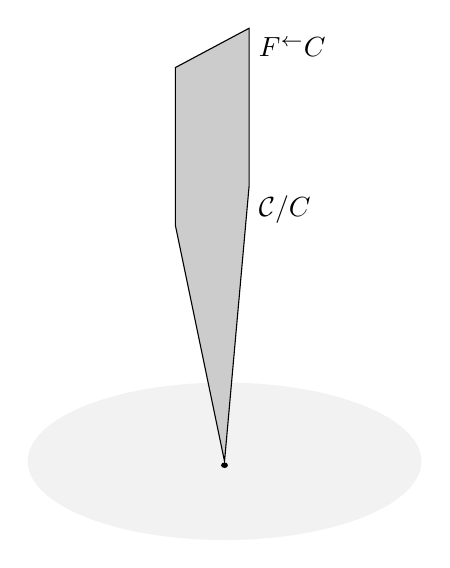
\begin{tikzpicture}[xscale=1.25]
    \fill[gray!10] (0,0) ellipse (2cm and 1cm);
    \filldraw[fill=gray!40, draw=black] (0,0) -- ++(-.5,3) -- ++(0,2) -- ++(.75,.5) node[below right] {$F^\leftarrow C$} -- ++(0,-2) node[below right] {$\mathcal{C}/C$} -- cycle;
    \fill (0,-.05) circle (1pt);
  \end{tikzpicture}
\end{document}